
\chapter{Introduction}
The primary content of my thesis is the four papers included in the thesis. This chapter is meant as a brief introduction to the background needed to understand the basics of the methods used throughout the papers. As such, this chapter is not meant to be a comprehensive guide to statistics and bioinformatics used in the papers. The original research motivation supporting the funding of this Ph.D. was multi-disciplinary and the papers included in my thesis are also highly influenced by this.

In \autoref{section:ancientDNA}, I will shortly introduce the field of ancient genomics and the statistical methods used to identify ancient DNA will be explained. Paper I, see \autoref{chapter:metadmg}, utilize modern Bayesian methods to classify which species are ancient, and which ones are not. Bayesian methods are great when possible, however, they also rely on some statistical model being defined. In the case of Paper I, the model is a beta-binomial distribution combined with an exponential-decay damage model.

Sometimes the model is not known and the data generation process has to be inferred by other means. This is the case in Paper II, see \autoref{chapter:hospital}, where we utilize machine learning methods to extract this information. This paper deals with estimating the individual risk scores for each patient being re-hospitalized after a knee or hip operation. \autoref{section:machine-learning} introduces the reader to basic classification with machine learning models.

While the former two papers are based on real life data, Paper III, see \autoref{chapter:covid19-agent-based-model}, concerns the development of a new agent based model for COVID-19. The model is based on the SIR model, but with a more detailed description of the disease and the transmission process. The model is used to simulate the spread of the virus in Denmark and to estimate the effect of contact tracing. The model is also used to simulate and predict the spread of the ``alpha'' variant of COVID-19 in Denmark. \autoref{section:agent-based-models} introduces the reader to the basics of agent based models.

Finally, the method of Bayesian model comparison of different diffusion models is introduced in Paper IV, see \autoref{chapter:diffusion}. In particular, this paper deals with different mixture-models of independent Rayleigh-distributions, and how they can be used to extract important information about the underlying diffusion processes of a polymer bridging model in cell nuclei, see \autoref{section:diffusion}.




\section{Ancient DNA and Bayesian Statistics}
\label{section:ancientDNA}


The similarity between family members and the degree to which siblings resemble one another has long been a mystery in human history.
People have always thought about the balance between nature and nurture, as in the famous fairy tale ``The Ugly Duckling'' by Hans Christian Andersen from 1843. These questions were addressed two decades later, when Gregor Mendel founded genetics as a modern, scientific discipline with his studies on trait inheritance in pea plants \autocite{mendelgregorVersucheUberPflanzenhybriden1866}.

A century later, a major breakthrough occurred when Watson and Crick discovered the double helix structure of DNA \autocite{watsonMolecularStructureNucleic1953}. This lead to other important discoveries within genetics, such as the development of DNA sequencing allowing scientists to identify the genetic makeup for a specific cell. Until the mid 1980s, studies within archaeogenetics were limited to analysis of fossilised samples of plants, animals or other species \autocite{parducciAncientDNAUnlocking2004}. Following the first successful recovery of ancient DNA from 5000 year old ancient Mummies, it was shown that it was indeed possible to extract and sequence DNA \autocite{paaboMolecularCloningAncient1985,paaboPreservationDNAAncient1985}.
This discovery, along with a dozen other, pushed the boundary for what is scientifically possible with ancient DNA, and led to Svante Pääbo being awarded with the Nobel Prize in Physiology or Medicine in 2022 for ``his discoveries concerning the genomes of extinct hominins and human evolution'' \autocite{thenobelassemblyatkarolinskainstitutetNobelPrizePhysiology2022}.

The field of ancient DNA (aDNA) was drastically changed with the invention of the Polymerase Chain Reaction (PCR) method \autocite{mullisSpecificEnzymaticAmplification1986} along with the Next Generation Sequencing (NGS) technology which revolutionized the speed and throughput of genomic sequencing, while decimating the cost \autocite{slatkoOverviewNextGeneration2018}. This technological advance has lead to better understanding of human migration and the genealogical tree of modern humans including the previously unknown human (sub)species; the Denisova hominin \autocite{krauseCompleteMitochondrialDNA2010}. In 2008, the first human genome was sequenced and since then multiple NGS methods have allowed for cheap, high-quality, in-depth sequencing of genetical samples \autocite{genomicsBriefHistoryNext2021}. All of this shows, that the field of genetics has grown exponentially and become a central part of modern biology.

Leaving the homocentric world view, aDNA also allows for the study of archaic animals. The age limitation for when aDNA can be sequenced has in the recent years increased; in 2013 with the early Middle Pleistocene \qtyrange[range-phrase = --,range-units = single]{560}{780}{\kilo\year\BP} horse \autocite{orlandoRecalibratingEquusEvolution2013} and in 2021 with the million-year-old mammoths \autocite{vandervalkMillionyearoldDNASheds2021}. High-throughput sequencing not only allows for the sequencing of single genomes -- like single humans, animals, or plants -- but also for sequencing of entire communities of organisms, so-called metagenomics. By analysing environmental DNA (eDNA) from a set of samples, one can survey the rich plant and animal assemblages of a given area and at a specific time in the past. Our new paper in Nature shows it is now possible to perform metagenomic sequencing on environmental DNA that is 2 million years old, see \autoref{appendix:kapk}. This is a direct application of the statistical method developed in Paper I, see \autoref{chapter:metadmg}, showing that \metaDMG can help to push the boundary of what is possible with ancient DNA.

Ancient DNA is difficult to work with since it often contains only a limited amount of biological material due to bad preservation, leading to low endogenous content with high duplication rates, making high-depth sequencing difficult\sidenote{Genotype likelihoods are often used to alleviate the problem of low-coverage data \autocite{nielsenGenotypeSNPCalling2011}.} \autocite{renaudAuthenticationAssessmentContamination2019}. Here endogenous content refers to DNA from the species of interest and not e.g. ancient bacteria or modern contamination.
In addition to this, ancient DNA is often highly degraded. In particular, the two prominent issues with aDNA is fragmentation and deamination \autocite{dabneyAncientDNADamage2013,peyregnePresentDayDNAContamination2020,}. Fragmentation refers to the fact that through time the DNA is broken into very short fragments, often with a size of less than \SI{50}{\basepairs}.
A consequence of this, upon alignment, is low mapping quality, multimapping, and reference bias, which can somewhat be mitigated by the use variant graphs \autocite{martinianoRemovingReferenceBias2020}.

\begin{figure}[htbp]
    \sidecaption{
        Illustration of DNA damage. Ancient DNA is often highly fragmented with short reads compared to modern, present-day DNA. Due to deamination, aDNA can contain uracils (U), which will be misread as thymines (T) while sequencing, leading to C-to-T nucleotide misincorporations. This is primarily happening at the end of the reads. Modified from \cite{peyregnePresentDayDNAContamination2020}.
        \label{fig:dna-damage-overview}}
    \centering
    \includegraphics[trim={0mm 90mm 0mm 90mm}, clip, width=\textwidth]{figures/illustrator/dna-deamination.pdf}
\end{figure}

Deamination is a process in which cytosine (C) in the single-stranded overhangs in the end of the DNA molecules is often hydrolized to uracil (U) which is read as thymine (T) by the DNA polymerase. This particular type of postmortem damage is known as cytosine deamination, or C-to-T transitions, and is one of the main reasons behind nucleotide misincorporations in ancient DNA \autocite{briggsPatternsDamageGenomic2007}. Due to the short fragment sizes in ancient DNA, the fragments will often contain overhangs with over-expressed C-to-T frequency. In the case of single-genome analysis, previous solutions have been to either remove all transitions and only keep transversions, apply trimming at the read ends, or enzymatically remove them with USER treatment \autocite{schubertImprovingAncientDNA2012,rohlandPartialUracilDNAglycosylaseTreatment2015}.
For an illustration of both fragmentation and deamination of ancient DNA, see  \autoref{fig:dna-damage-overview}.

Measuring DNA damage is thus a way to prove authentic aDNA. Currently, a handful of different methods for quantifying ancient DNA damage exist. In particular, the mapDamage software has been the standard for how to measure ancient DNA damage in the field \autocite{jonssonMapDamage2FastApproximate2013}. While mapDamage allows for estimating all of the four Briggs parameters, it is often the empirical deamination patterns that mapDamage computes that are used. Newer and faster methods for estimating ancient DNA damage are continuously being developed, including PyDamage \autocite{borryPyDamageAutomatedAncient2021}, which tackles some of mapDamage's limitations. However, within metagenomics, which studies the genetic material of all organisms collected from an environmental sample, faster methods suited to analyse this large-scale dataset are still lacking.

Paper I, see \autoref{chapter:metadmg}, introduces the \metaDMG software which utilizes the C-to-T deamination pattern\sidenote{for the forward strand and the G-to-A deamination pattern for the reverse strand.} to identify ancient DNA damage. One of the key features of this method is the beta-binomial model which allows the uncertainty of the deamination frequency to be fitted independently of the mean of the frequencies leading to improved accuracy of the damage estimation. The deamination frequencies are based on the number of C-to-T transitions, $k$, out of the total number of C's, $N$, for a given position within the fragment. The classical likelihood to use for this type of data is a binomial distribution. The mean and variance of the binomial distribution is given by:
\begin{equation}
    \begin{split}
        \EX{k}  &= N p \\
        \VarX{k} &= Np(1-p),
        \label{eq:Binomial_expectation_variance}
    \end{split}
\end{equation}
where $p$ is the probability of success (a C-to-T substitution). One of the issues, however, is that the variance of the binomial distribution is proportional to the mean. The binomial distribution is thus not flexible enough to accommodate large amounts of variance in the data, so-called overdispersion \autocite{mcelreathStatisticalRethinkingBayesian2020}. One way to accommodate overdispersion is to instead use a beta-binomial model. The beta-binomial model is a generalization of the binomial distribution where the variance is independent of the mean. Technically, the beta-binomial model assumes that $p$ is a random variable which follows a beta distribution $p \sim \mathrm{Beta}(\mu, \phi)$ where the beta distribution is parameterized\sidenote{This can be reparameterization in term of the classical $\alpha, \beta$ parameterization by: $\mu = \alpha / (\alpha + \beta)$ and $\phi = \alpha + \beta$.} in terms of its mean, $\mu$, and dispersion parameter, $\phi$, \autocite{cepeda-cuervoDoubleGeneralizedBetaBinomial2017}. The mean and variance of this beta-binomial model is then given by:
\begin{equation}
    \begin{split}
        \EX{k}  &= N \mu \\
        \VarX{k} &= N\mu(1-\mu) \frac{\phi+N}{\phi+1}.
        \label{eq:BetaBinomial_expectation_variance}
    \end{split}
\end{equation}

Comparing \autoref{eq:Binomial_expectation_variance} and \autoref{eq:BetaBinomial_expectation_variance}, it is seen that the variance of the beta-binomial model is no longer (strictly) proportional to the mean, but instead is a function of the dispersion parameter, $\phi$, allowing for higher variance than the binomial-only model. When $\phi = 0$, the variance of the beta-binomial model is $N$ times larger, and when $\phi \rightarrow \infty$ the variance reduces to the variance of the binomial model, showing that the beta-binomial model is a generalization of the binomial model.

\autoref{eq:BetaBinomial_expectation_variance} shows how to model the C-to-T damage at a specific base position in the read. We model the position-dependent damage frequency, $f(x) = k(x) / N(x)$, see \autoref{fig:dna-damage-overview}, as a function of the distance from the end of the read, $x$, with a modified geometric damage profile (exponential decay):
\begin{align}
    y(x; A, q, c) = A(1-q)^{x-1} + c.
    \label{eq:damage_function}
\end{align}
Here $A$ is the scale factor, or amplitude, $q$ is the decay rate, and $c$ is a constant offset. The offset can be interpreted as the baseline C-to-T background substitution rate or baseline damage rate. Since $x$ is discrete, this is similar to a (modified) geometric sequence starting from $x=1$. The combination of equation \eqref{eq:BetaBinomial_expectation_variance} and \eqref{eq:damage_function} is illustrated in \autoref{fig:damage-model-sketch}, which shows the position-dependent decreasing damage frequency. The figure also shows the increase in uncertainty in the beta-binomial model compared to the binomial-only model.
\begin{figure}[htbp]
    \sidecaption{
        Illustration of the damage model. The figure shows data points as circles and the fitted damage frequency, $y(x)$, as a solid line. The amplitude of the damage is $A$, the offset is $c$, and the relative decrease in damage pr. position is given by $q$. The damage uncertainty for a binomial model is shown in dark grey and the uncertainty for a beta-binomial model in light grey.
        \label{fig:damage-model-sketch}}
    \centering
    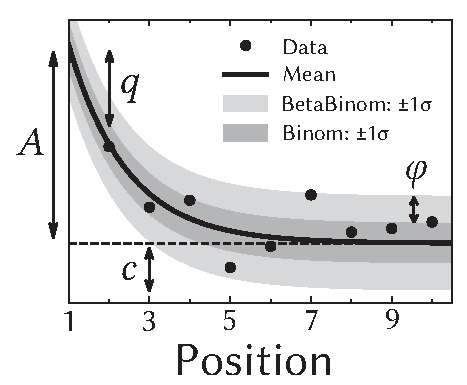
\includegraphics[width=0.6\textwidth]{figures/damage_sketch_new.pdf}
\end{figure}

The damage framework described above is based on the nucleotide misincorporations, i.e. the C-to-T transitions. The background for this data can be from either DNA sequence files mapped to a single genome or from metagenomic data consisting of multiple mapped reads. As such, the damage framework is a general tool for estimating damage based on DNA alignment files.

In the metagenomic case, \metaDMG identifies the lowest common ancestor (LCA) based on the algorithm from ngsLCA \autocite{wangNgsLCAToolkitFast2022}.
For each read that maps to multiple reference genomes from separate species, i.e. has multiple alignments, the taxonomic tree is traversed for each alignment until a common ancestor is found. \autoref{fig:tree-LCA} illustrates the LCA for a read that maps to different (sub)species. In this example, the LCA of alignment 1 and 2 is the Subspecies I while the LCA for all four alignments is the Genus X. \metaDMG works by default with the NCBI taxanomic database but can also be used with custom databases.

\begin{figure}[htbp]
    \sidecaption{
        Illustration of the lowest common ancestor (LCA) for taxonomic trees. Here the LCA of alignment 1 and 2 is Subspecies I, while the LCA of all four reads is Genus X. The dots ($\dots$) refers to other taxonomic levels, e.g. family and order.
        \label{fig:tree-LCA}}
    \centering
    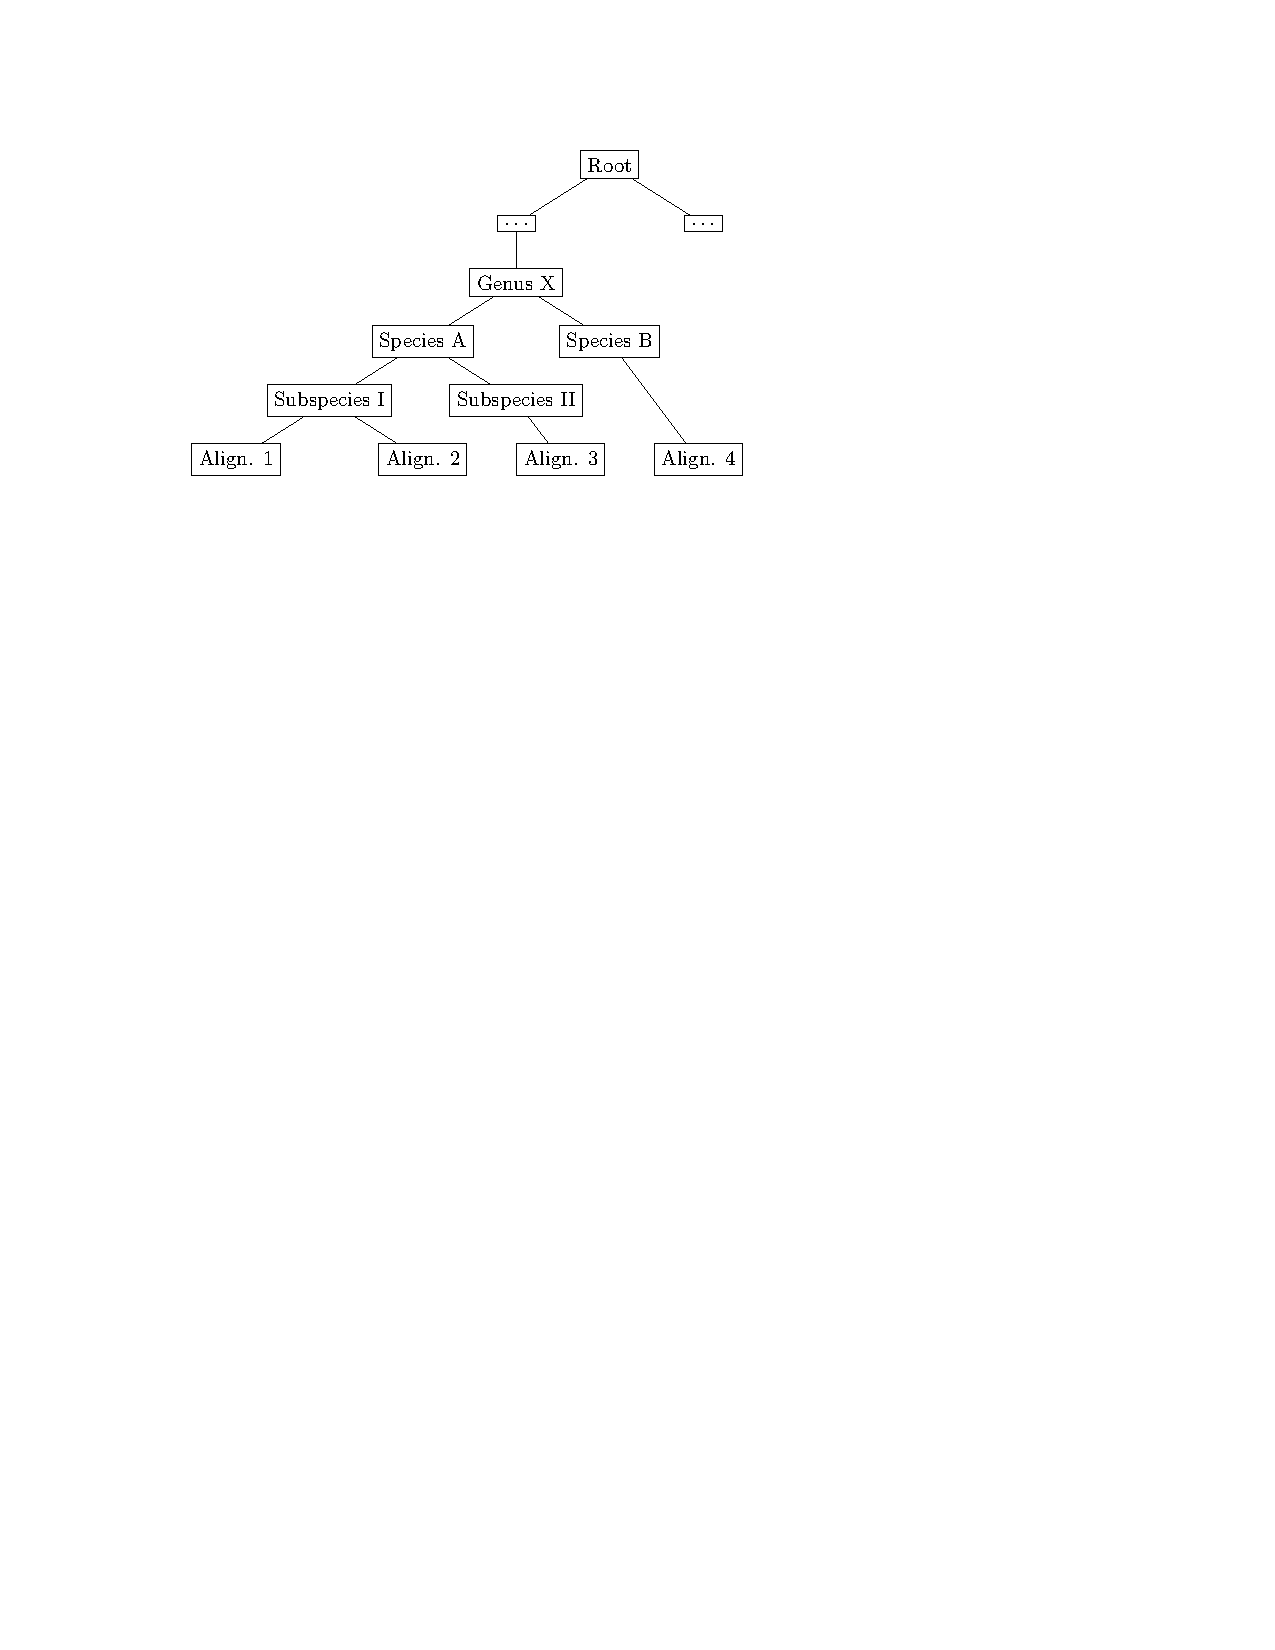
\includegraphics[trim={3cm 19.5cm 8.5cm 2.3cm}, clip, width=0.8\textwidth]{figures/tree.pdf}
\end{figure}

Given the nucleotide misincorporations, either coming from a single-reference alignment file or after LCA in the metagenomic case, eq. \eqref{eq:BetaBinomial_expectation_variance} and \eqref{eq:damage_function} are fitted with a Bayesian model. This is done to ensure the optimal inference of the parameters, $A$, $q$, and $c$, and to account for the uncertainty in the data. Bayesian inference also allows for the inclusion of domain knowledge in the form of the prior distribution by Bayes theorem. Bayes theorem is based on the law of conditional probability \autocite{barlowStatisticsGuideUse1993} stating that the probability of two events, $A$ and $B$, both happening, $P(A \cap B)$, is given by:
\begin{align}
    P(A \cap B) = P(B)P(A|B),
    \label{eq:bayes_theorem_1}
\end{align}
where $P(B)$ is the probability of $B$ and $P(A|B)$ is the conditional probability of $A$ given $B$. Similarly, $P(A \cap B)$ can also be expressed in terms of the probability of $A$:
\begin{align}
    P(A \cap B) = P(A)P(B|A).
    \label{eq:bayes_theorem_2}
\end{align}
Combining \autoref{eq:bayes_theorem_1} and \autoref{eq:bayes_theorem_2} and rearranging terms gives the Bayes theorem:
\begin{align}
    P(\theta|D) = \frac{P(\theta)P(D|\theta)}{P(D)},
    \label{eq:bayes_theorem}
\end{align}
with a change of variables where $D$ refers to the observed data and $\theta$ the parameter(s) of the model\sidenote{In the case of \metaDMG, $D$ would be the observed deamination frequencies and $\theta$ the four fit parameters.}. The first term in the numerator, $P(\theta)$, is the prior distribution and describes the probability distribution assigned to $\theta$ before observing any data. The second term is the likelihood function, $P(D|\theta)$, which is the probability of observing the data given the parameter(s). Together these two terms combine to a compromise between data and prior information.

The numerator, $P(D)$, also known as the evidence, can be treated as a data-related normalization factor. In the case of continuous $\theta$, this can calculated as the marginalization of the likelihood function over $\theta$:
\begin{align}
    P(D) = \int_\theta P(D|\theta)P(\theta) \dx \theta.
    \label{eq:evidence}
\end{align}
This equation, however, is often intractable to compute in the higher-dimensional case. Luckily, it can be shown that Markov Chain Monte Carlo (MCMC) sampling can approximate the posterior distribution, $P(\theta|D)$, and asymptotically converge to the correct distribution \autocite{gelmanBayesianDataAnalysis2015a}.

Traditionally MCMC methods such as Metropolis Hastings (MH) or Gibbs sampling have been used for Bayesian inference, however, these methods are often slow and require a lot of tuning. In the last decades, a new class of MCMC methods have been developed, namely Hamiltonian Monte Carlo (HMC) methods. While traditional MH uses a Gaussian random walk, HMC is a gradient-based MCMC method that uses Hamiltonian dynamics to guide the sampling. This makes HMC more efficient than traditional MCMC methods and allows for sampling from high-dimensional distributions \autocite{betancourtConceptualIntroductionHamiltonian2018,nealMCMCUsingHamiltonian2011}. A particularly efficient type of HMC is the No-U-Turn Sampler (NUTS). NUTS is a variant of HMC that automatically tunes the step size and number of steps to take in the Hamiltonian dynamics \autocite{homanNoUturnSamplerAdaptively2014}.

Most statistical domain-specific languages (DSL) such as Stan \autocite{carpenterStanProbabilisticProgramming2017}, Pyro \autocite{binghamPyroDeepUniversal2019}, NumPyro \autocite{phanComposableEffectsFlexible2019} or Turing.jl \autocite{geTuringLanguageFlexible2018}, implement HMC and in particular the NUTS algorithm. Since the statistical modelling part of \metaDMG is implemented in Python, NumPyro is used for the Bayesian inference of the damage model, as it is easy to implement and computationally efficient since it uses JAX \autocite{bradburyJAXComposableTransformations2018} under the hood for automatic differentiation and just-in-time (JIT) compilation.

Even though NumPyro is fast and \metaDMG is efficiently implemented, the Bayesian inference of the damage model is still computationally expensive. Thus, it was decided to also include a faster, approximate method of Bayesian inference: the maximum a posteriori (MAP) estimate. The MAP estimate is the point estimate of the posterior distribution that maximizes the posterior probability density function, i.e. the posterior mode:
\begin{align}
    \hat{\theta}_\mathrm{MAP} = \argmax_\theta P(\theta|D) = \argmax_\theta P(\theta)P(D|\theta),
\end{align}
where the second equality is due to the evidence being independent of $\theta$. Since this is a point estimate, $\hat{\theta}_\mathrm{MAP}$ does not fully explain the full posterior, however, it is often a good approximation\sidenote{Especially when the posterior is unimodal, which is generally the case for \metaDMG.}. Comparing $\hat{\theta}_\mathrm{MAP}$ to the maximum likelihood estimate (MLE):
\begin{align}
    \hat{\theta}_\mathrm{MLE} = \argmax_\theta P(D|\theta),
\end{align}
the MAP estimate can be seen as a regularized version of the MLE estimate \autocite{murphyMachineLearningProbabilistic2012}. To further optimize the computational efficacy of the MAP estimation in \metaDMG, the MAP estimation function is JIT compiled using Numba \autocite{lamNumbaLLVMbasedPython2015} and mathematically optimized with iMinuit \autocite{dembinskiScikithepIminuitV22021}.

% One of the limitations of the \metaDMG software is XXX.



\section{Anestesiology -- a Machine Learning Approach }
\label{section:machine-learning}

This section explains the technical background behind Paper II, see \autoref{chapter:hospital}. This study investigates the potential advantages of using a modern machine-learning model compared to classical logistic regression to predict the risk of patients being re-hospitalized after fast-track hip and knee replacements. In particular, the patients were grouped into two groups where the ``risk-patients'' all stayed in the hospital for more than four days after the operation or were readmissioned to the hospital within 90 days after the operation. As such, this is a binary classification problem where the patient's risk-score is predicted based on historical data.

Most classification and regression problems fall under the same machine learning (ML) branch called supervised learning. In supervised learning, the goal is to find the optimal hypothesis $h^*$ in the hypothesis set $\mathcal{H}$ that matches the unknown, ``true'' data-generating function $f: \mathcal{X} \rightarrow \mathcal{Y}$ as good as possible, where $\mathcal{X}$ is the input space and $\mathcal{Y}$ is the output space. Assuming that we have access to realizations of $f$, the so-called training data $\mathcal{D}_\mathrm{train} = \{(\mathbf{x}_i, y_i)\}_{i=1}^N$, we can use a learning algorithm $\mathcal{A}$ combined with the training data to estimate $h^*$ \autocite{abu-mostafaLearningData2012a}. Here $N$ refers to the number of training samples and $\mathbf{x}_i$ is the $i$th observation with the true label $y_i$. This process is illustrated in \autoref{fig:ML-setup}.

\begin{figure}[htbp]
    \sidecaption{
        Illustration of how to learn from data in a supervised learning setting. Adapted from \autocite{abu-mostafaLearningData2012a}.
        \label{fig:ML-setup}}
    \centering
    \includegraphics[width=0.9\textwidth]{figures/illustrator/ML-learning.pdf}
\end{figure}

Both the logistic regression (LR) and ML model can be viewed through the lens of \autoref{fig:ML-setup}, just with $|\mathcal{H}_\mathrm{LR}| \ll |\mathcal{H}_\mathrm{ML}|$, i.e. the machine learning model is a lot more complex than the logistic regression model\sidenote{And the hypothesis space thus is significantly larger.}. To predict the performance of $h^*$ on new, unseen data, the naive method would be to train on all of the data and evaluate on the same, however, this would have a high risk of overfitting the data and thus biasing the predicted performance\sidenote{Especially for high cardinality hypothesis sets.} \autocite{abu-mostafaLearningData2012a}.

To avoid this and get more accurate estimates of the performance of $h^*$, we use a technique called cross-validation (CV). In the simplest way, this can be done by splitting the data into two sets, one called the training and one called the validation set, and then only train on the training set. Afterwards the trained model can be evaluated on the validation set without biasing the performance estimate. This process can further be refined by splitting the data into $K$ folds and then repeating the process $K$ times, where each fold is used as the validation set once.
This is called $K$-fold cross-validation and is illustrated in \autoref{fig:ML-crossval-kfold} \autocite{murphyMachineLearningProbabilistic2012,hastieElementsStatisticalLearning2016}.
$K$-fold cross validation works well in many cases, yet in the case of temporal data, it also risks introducing bias in the performance estimates, since, in the different folds, it, effectively, is allowed to ``look into the future''. The most extreme case of this is shown in the bottom of \autoref{fig:ML-crossval-kfold} where the model trains on all future and present data and is then evaluated only on past data. In many time dependent datasets, this is undesirable. Instead, we use a technique called temporal cross validation \autocite{tashmanOutofsampleTestsForecasting2000a}, see \autoref{fig:ML-crossval-temporal}, which circumvents this problem by only allowing the model to train on past data and evaluate on future data. As the patient data is time dependent\sidenote{The fraction of rehospitalizations decreased over time due to surgerilogical improvements.}, this is the technique we use in Paper II.

\begin{figure}[htbp]
    \centering
    \sidecaption{
        Two types of cross validation: $K$-fold cross validation, and temporal cross validation. Both figures from \cite{michelsenPhysicistApproachMachine2020}.
        \label{fig:ML-crossval}}
    \begin{subfigure}{.5\textwidth}
        \centering
        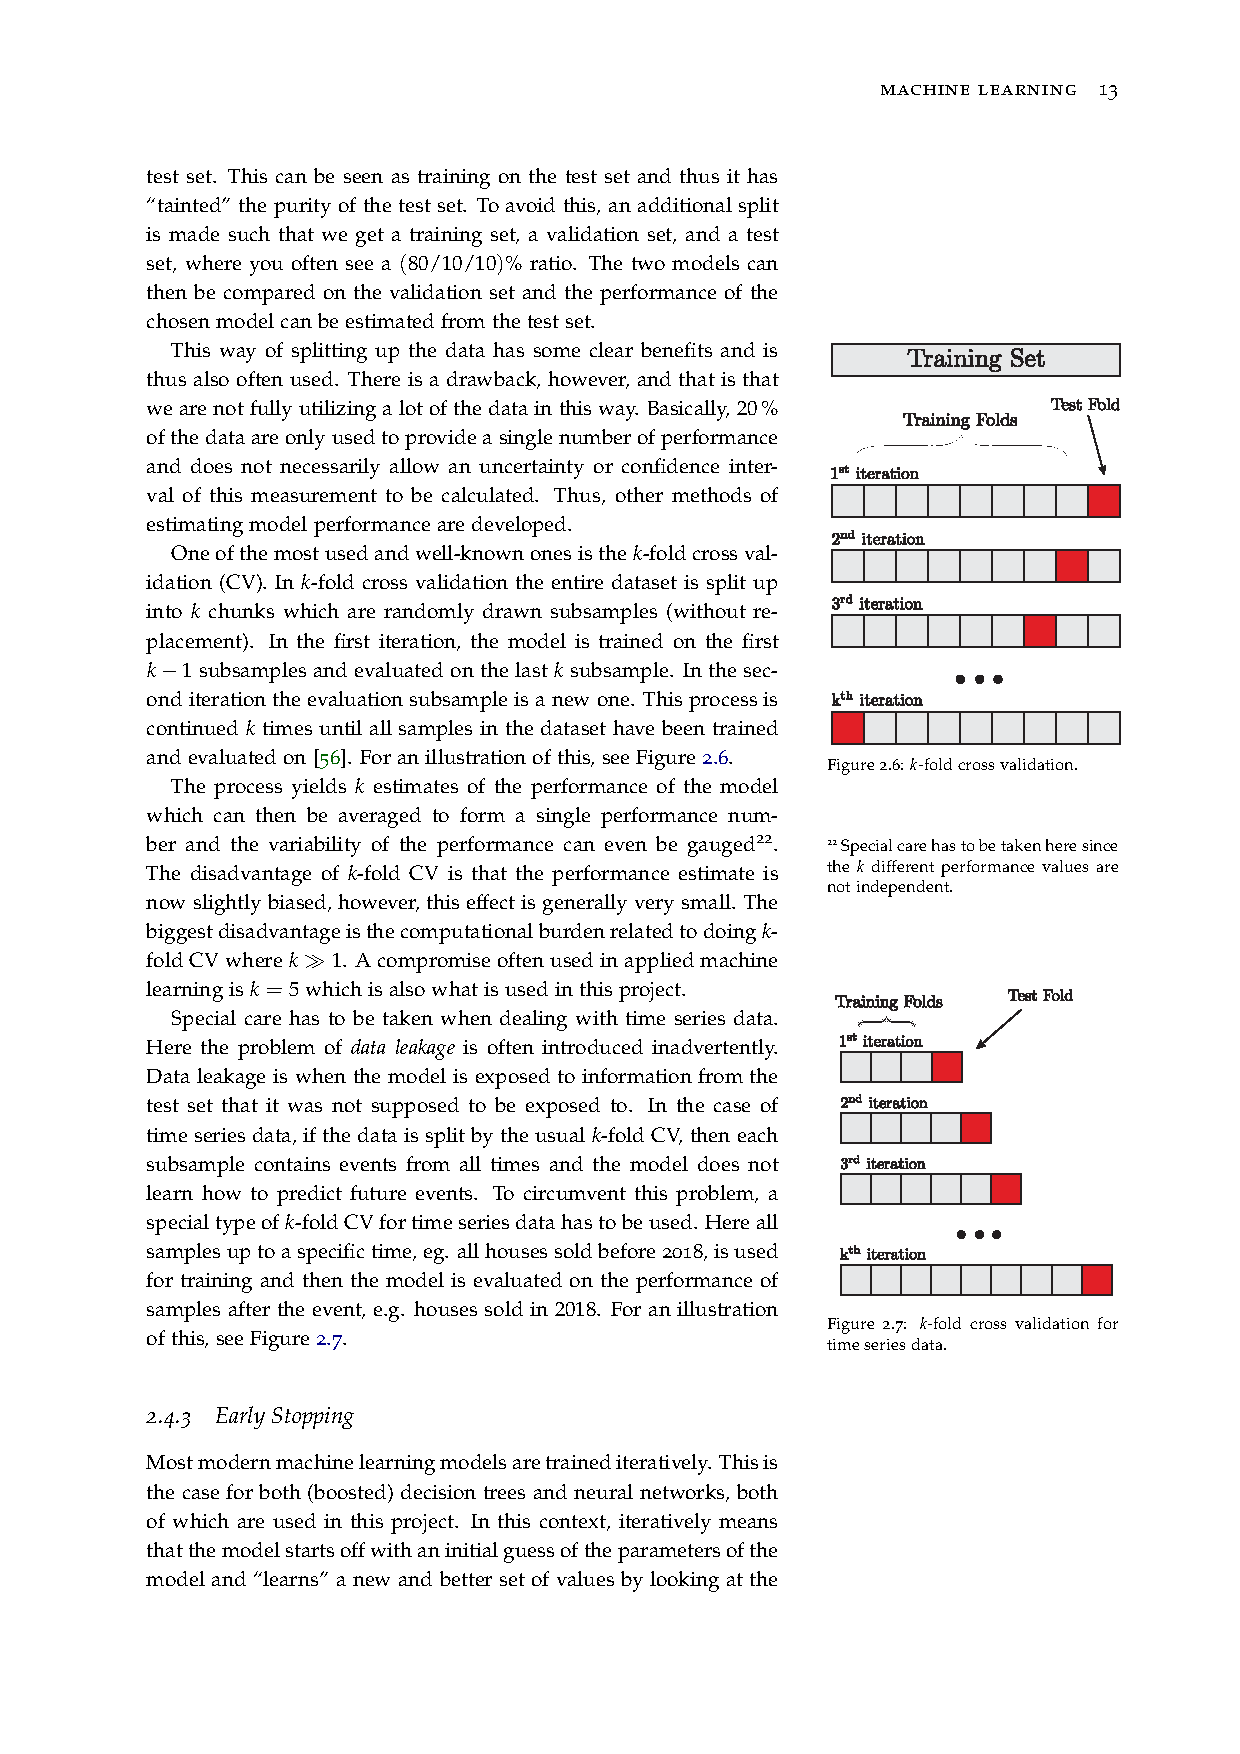
\includegraphics[trim={14cm 17cm 1.95cm 6.5cm}, clip, width=.8\linewidth]{figures/MasterThesis-cross-validation}
        \caption{$K$-fold cross validation}
        \label{fig:ML-crossval-kfold}
    \end{subfigure}%
    \begin{subfigure}{.5\textwidth}
        \centering
        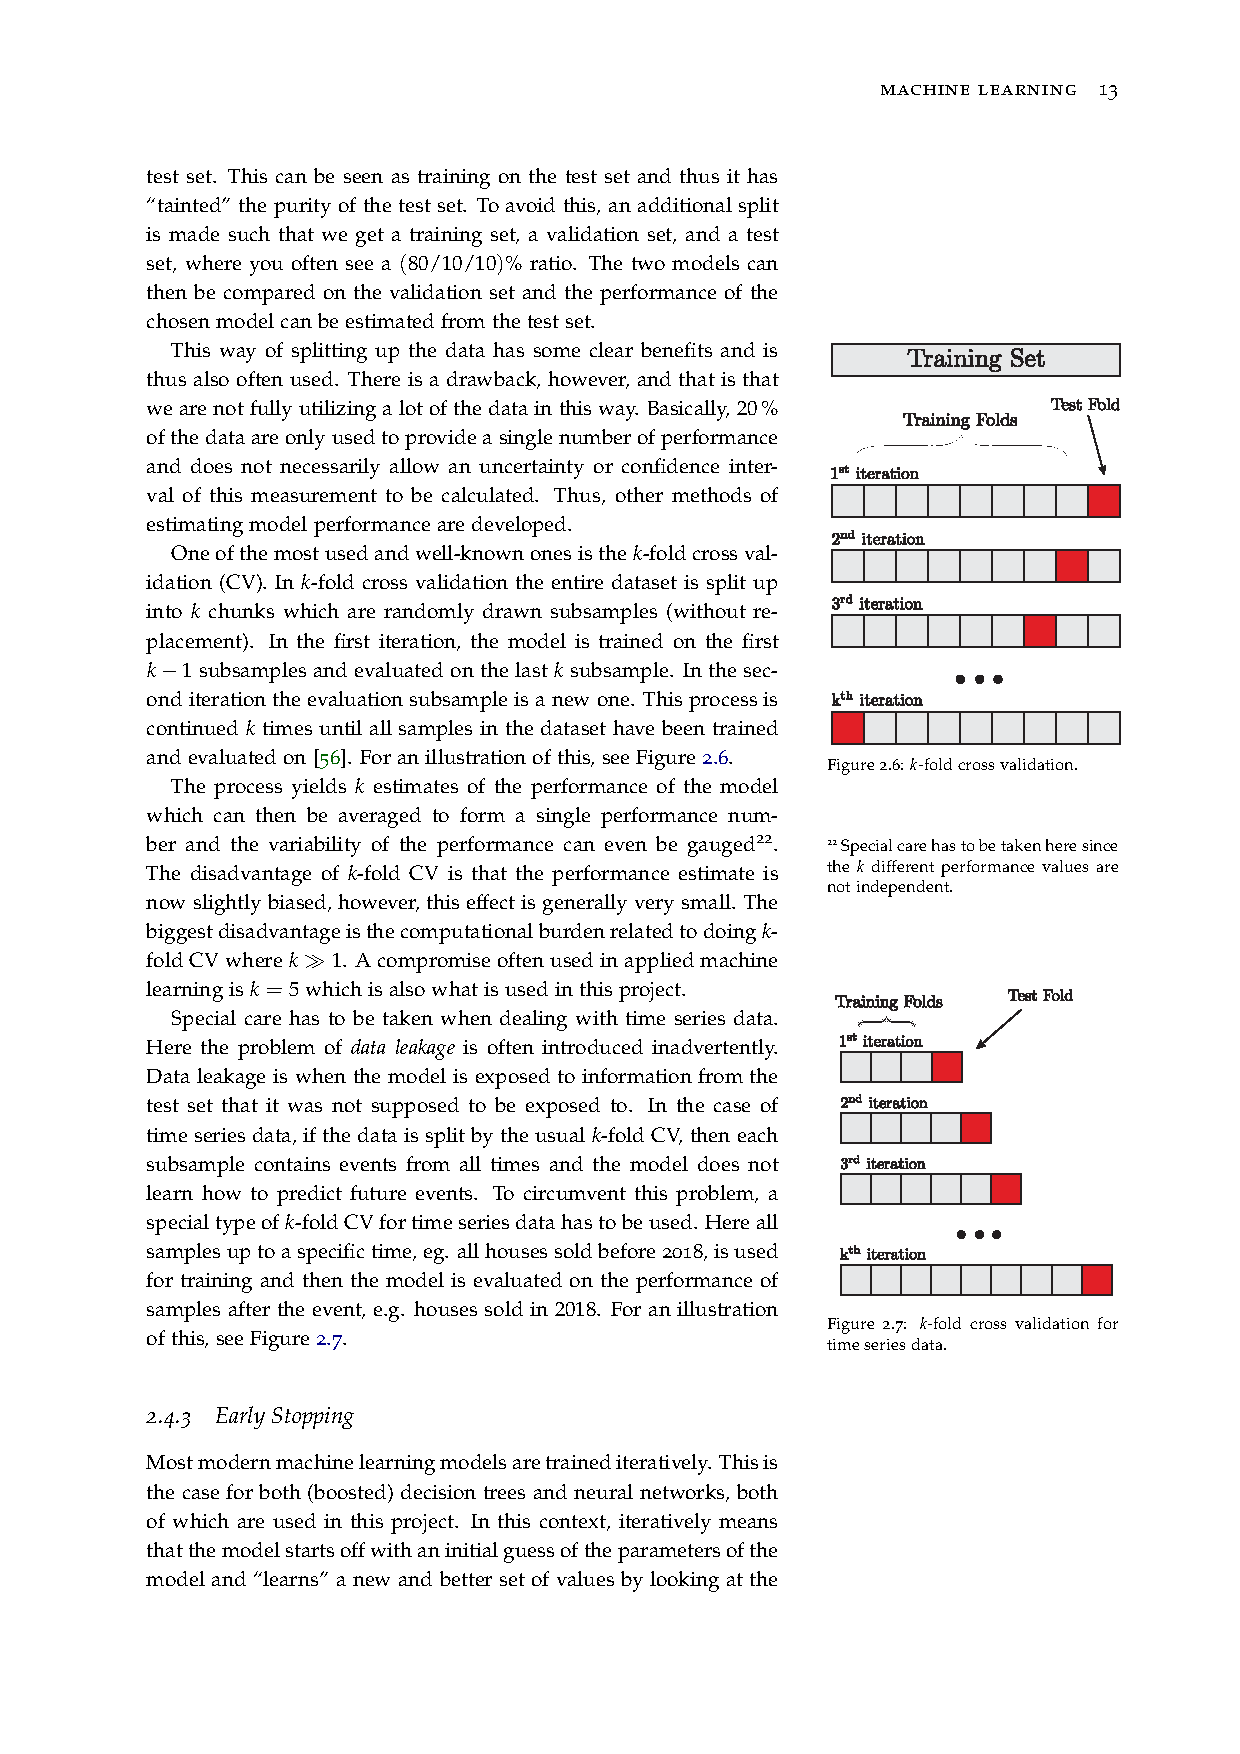
\includegraphics[trim={14.14cm 7.67cm 2.1cm 16.5cm}, clip, width=.8\linewidth]{figures/MasterThesis-cross-validation}
        \caption{Temporal cross validation}
        \label{fig:ML-crossval-temporal}
    \end{subfigure}
\end{figure}

The training of the learning model $\mathcal{A}$ itself is model-dependent and will not be covered in this thesis, see \autocite{michelsenPhysicistApproachMachine2020} for a more detailed description of the training process. This is not the only way to optimize the performance of  $\mathcal{A}$, albeit it is the primary one. In addition to the internal parameters of the model, some parameters are external to the model in the sense that they are not optimized by the model itself, but rather by the user. These are called hyperparameters and are often optimized using a technique called hyperparameter optimization (HPO). In the case of logistic regression, the number of variables to include would be an example of a hyperparameter; in the case of a decision tree model, the depth of the tree. Hyperparameter optimization can be performed in many ways, where the classical one is through grid search, see \autoref{fig:ML-hpo-GS}.
\marginfig{figures/MasterThesis-hpo-grid.pdf}{Illustration of grid search. Figure from \cite{michelsenPhysicistApproachMachine2020}.}{fig:ML-hpo-GS}

In grid search all combinations of the hyperparameters (the cartesian product) are tried and the best combination is chosen. This is a simple and intuitive approach, however, it scales exponentially, i.e. very poorly, with the number of hyperparameters\sidenote{As such, grid search suffers from the curse of dimensionality.}. In addition to this, it depends on the user-defined grid, which might not be optimal. To circumvent this, a technique called random search (RS) was developed \autocite{bergstraRandomSearchHyperparameter2012a}. Random search is a randomized version of grid search, where the hyperparameters are sampled randomly from a distribution. This allows for a more efficient sampling of the hyperparameter space, see \autoref{fig:ML-hpo-RS}, and further lets the user decide on the number of iterations beforehand.

\marginfig{figures/MasterThesis-hpo-random.pdf}{Illustration comparing grid search to random seach. The height of green surve is the score-function which has to be optimized. Figure adapted from \cite{bergstraRandomSearchHyperparameter2012a}.}{fig:ML-hpo-RS}

The disadvantage of random search is that all draws are fully independent. While this allows for easy parallelisation of the algorithm, this also means that each new sample might be infinitesimal close in the hyperparameter space to a previous sample with bad performance, which with high probability will thus also have a high loss. An approach that does take the history of the previous samples' performance into consideration is Bayesian optimization \autocite{brochuTutorialBayesianOptimization2010a}. In Bayesian optimization each successive hyperparameter is chosen based on an acquisition function which optimizes the expected improvement in the performance of the model. This is illustrated in \autoref{fig:ML-hpo-BO}. This leaves the user with the task of choosing between ``exploitation'' and ``exploration'' of the hyperparameter space in the definition of the acquisition function, yet most implementations of bayesian optimization have decent default settings.

\begin{figure}[htbp]
    \sidecaption{
        Illustration of the learning process of Bayesian optimization. The previous observations are shown as black dots and the true objective function is shown as a dashed black line. This line is fitted with Gaussian processes which is shown as the solid line with its uncertainty in purple. The acquisition function is shown in green and its maximum decides what the next iteration of the hyperparameter value(s) should be \autocite{michelsenPhysicistApproachMachine2020}.
        \label{fig:ML-hpo-BO}}
    \centering
    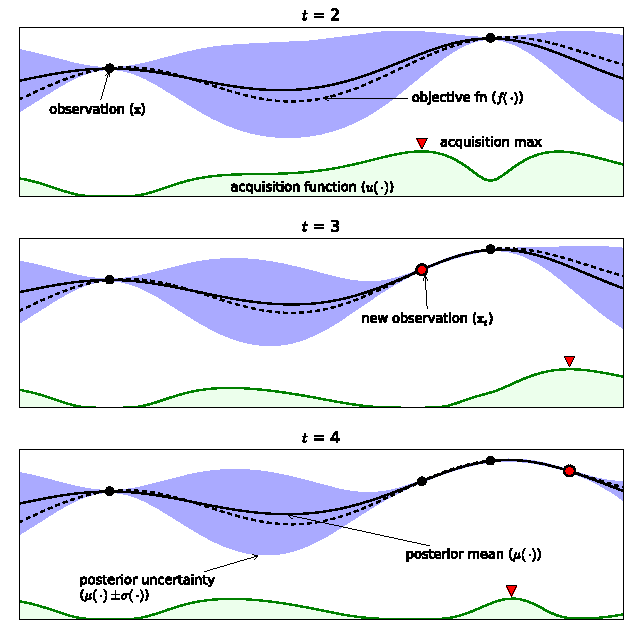
\includegraphics[width=0.7\textwidth]{figures/MasterThesis-hpo-bayesian}
\end{figure}

We use the Python package Optuna \autocite{akibaOptunaNextgenerationHyperparameter2019} for HPO in Paper IV due to its ease of use and its support for Bayesian optimization. In particular, we use the Tree-structured Parzen Estimator algorithm for the Bayesian optimization and a median stopping rule to minimize optimization time \autocite{bergstraAlgorithmsHyperParameterOptimization2011}. This allowed for a good comporise between optimization time and performance.

While model performance is often paramount, in some fields -- such as medicine -- being able to explain the model's predictions is almost as important. This is especially true in the case of medical decision support systems, where the model is used to make decisions about the patient's treatment. Model explainability helps to build trust in the model for both the patient and the medical staff alike.

In Paper II, we employ the SHapley Additive exPlanations (SHAP) values which provide estimates on which variables contribute most to the risk score predictions \autocite{lundbergUnifiedApproachInterpreting2017,lundbergLocalExplanationsGlobal2020}. SHAP values allow for not only a global explanation of the model, i.e. which features are most important overall, but also a local explanation, i.e. why a single patient was predicted to be at risk of being re-hospitalized. It has previously been shown that the interaction between SHAP values and medical doctors can improve the performance of anaesthesiologists  \autocite{lundbergExplainableMachinelearningPredictions2018a}.

While the aim of Paper II is to show how modern machine learning techniques can be used to improve the risk prediction process, the usefulness of the SHAP values in a medical context is demonstrated in the paper in \autoref{appendix:anaemia}. The paper uses the SHAP values to compare the preoperative haemoglobin level in the patient with the risk-score, stratified by sex and operation type (knee vs hip replacement). Currently, the WHO guidelines for the haemoglobin levels are gender specific \autocite{anaemiasNutritionalAnaemiasReport1968}, however, this study finds no significant gender difference and a haemoglobin threshold close to the WHO suggestions for men.

\section{COVID-19 and Agent Based Models}
\label{section:agent-based-models}
In early 2020, a contagious disease called COVID-19 started to spread in Europe, including Denmark. With new infections showing up faster and faster, governments started to implement different measures to limit the spread of the deadly disease, including lockdowns, travel restrictions, and social distancing, measures not previously seen in peacetime since the Spanish flu in 1918. This was the background for the work that we did in 2020 which became the basis for Paper III, see \autoref{chapter:covid19-agent-based-model}. This paper deals with the development of a new agent based model for COVID-19 in Denmark in collaboration with Statens Serum Institut (SSI), the Danish Center for Disease Control.

Historically, most mathematical models of infectious diseases were variations of the SIR model, which describe the evolution of a pandemic by approximating all individuals as one population \autocite{kermackContributionMathematicalTheory1927}.
As one of the simplest compartmental models, the susceptible-infectious-recovered (SIR) model is based on a system of three non-linear differential equations that describe the transition between each state, or compartment, of the model \autocite{krogerAnalyticalSolutionSIRmodel2020}. Initially the entire population is susceptible until time $t=0$ at which some individuals become not only infected, but also infectious, allowing the disease to spread. After having been infectious, the individuals recover and become immune to the disease and stop being infectious. Several variations of the SIR model exist, including the SIS model, where the recovered individuals become susceptible again \autocite{hethcoteThreeBasicEpidemiological1989}. Another variation is the SEIR model, which includes an exposed state, where individuals are infected but not yet infectious, which is the basis for the model used in Paper III.

SIR-like models suffer from several shortcomings, including the assumptions that the population is homogeneous, and that the disease is transmitted at a constant rate. In reality, neither the population nor the transmission rates are homogenous. These are some of the reasons why we chose to use an agent based model (ABM). Agent based models simulate individual agents in a population that can have complex interactions patterns, e.g. based on their geography \parencite{wilenskyIntroductionAgentBasedModeling2015}.

In particular, we implemented a continuous-time, stochastic, spatial ABM using the Gillespie algorithm, a stochastic simulation algorithm \autocite{gillespieExactStochasticSimulation1977}. The model is JIT compiled with Numba \autocite{lamNumbaLLVMbasedPython2015} to speed up the simulation, allowing the simulation of the Danish population of 5.8 million people in a couple of hours instead of days. The model allows for the individual tuning of the three main effects; A) heterogeneities in the infection strength\sidenote{allowing \emph{super-shedders}}, B) number of connections\sidenote{allowing \emph{super-connecters}}, C) and the spatial clustering of the agents. In the absence of any of these effects, we find that the ABM's predictions matches the SIR model's predictions within $\pm 5 \%$. Once we allowed for spatial clustering, we found that the epidemic developed faster and with a higher infection peak compared to the SIR model, but that the total number of infected in the end of the epidemic was lower.

In real-life scenarios, one does not have the opportunity to let the epidemic run loose and afterwards evaluate the strength of the epidemic; the goal is to predict the intensity in the very beginning of the epidemic and implement lockdown-related measured based on this estimate. In the second part of Paper III, we show that once spatial clustering is introduced, fitting standard SEIR-models to infection numbers from the first few days of the epidemic, predictions are overestimated by a factor of two. The results are a significant over-estimation of the impact of the epidemic. Since the population is highly susceptible in the beginning of an epidemic, this also highlights the benefits of early lockdowns to reduce the effect of the super connectors.

The developed ABM was further used by SSI to estimate the effect of contact tracing related to COVID-19 in Denmark, see \autoref{appendix:ssi-report}. It was further used to estimate spread of the ``alpha'' variant of COVID-19 (B.1.1.7) in Denmark, see \autoref{appendix:ssi-notat}. Based on data available January 2nd 2021, the model predicted that the ``alpha'' variant would be the dominant variant in Denmark February 10--20, 2021. It became the dominant variant in Week 7: February 15--21, 2021 \autocite{bagerRiskHospitalisationAssociated2021}.


\section{Diffusion Models and Bayesian Model Comparison}
\label{section:diffusion}

The similarity between family members and the degree to which siblings resemble one another has long been a mystery in human history.
People have always thought about the balance between nature and nurture, as in the famous fairy tale ``The Ugly Duckling'' by Hans Christian Andersen from 1843. These questions were addressed two decades later, when Gregor Mendel founded genetics as a modern, scientific discipline with his studies on trait inheritance in pea plants \autocite{mendelgregorVersucheUberPflanzenhybriden1866}.
% although it was not until a century later that Watson and Crick discovered the double helix structure of DNA .

A century later a major breakthrough was when Watson and Crick discovered the double helix structure of DNA \autocite{watsonMolecularStructureNucleic1953}. This lead to other important discoveries within genetics, such as the development of DNA sequencing allowing the scientist to identify the genetic makeup for a specific cell. In 2008, the first human genome was sequenced and since then multiple Next-Generation Sequencing methods (NGS) have allowed for cheap, high-quality, in-depth sequencing of genetical samples \autocite{genomicsBriefHistoryNext2021}. Since then, the field of genetics has grown exponentially and has become a central part of modern biology today.

While \autoref{section:ancientDNA} discusses the behaviour of ancient DNA, Paper IV focusses on how living cells work and, in particular, how they regulate the transcription of DNA in the cell nucleus.
Despite the fact that all cells share the same DNA, the regulation and expression of the genes stored within can vary. The mechanism of the cell-specific expression and silencing of specific genomic regions are one of the most fundamental biological challenges.

Currently, different biological models try to explain the physical principles creating the heterogeneous environment in the cell nucleus of eukaryotic cells.
One of these is the polymer-bridging model (PBM) that models the micro compartments called the foci. The cell nucleus contains two different types of loci; the repair foci and the silencing foci. Paper IV studies the physical mechanism of the formation of the silencing foci.

\autoref{fig:diffusion-model} illustrates the parts of the cell nucleus relevant to the polymer-bridging model. Inside the nucleus, DNA fibers are curled up and some parts of the DNA locate inside the silencing foci. Inside the silencing foci, the PBM predicts binding and bridging sites that interact with the DNA fiber through the SIR proteins, which is up-regulated inside the the region of the foci \autocite{heltbergPhysicalObservablesDetermine2021}. The silent Information Regulator (SIR) proteins repress the underlying genes, and, due to the increased concentration inside the focus, the foci are termed silencing foci.

\begin{figure}[htbp]
    \sidecaption{
        Illustration of the cell nucleus. The nucleus membrane is shown in red and the repair foci in yellow. The black line represents the DNA fiber which is curled up in the silencing foci in green. The right side of the figure shows a zoomed in view of the silencing foci according to the polymer-bridging model with the binding and bridging sites that interact with the SIR proteins. The tracking of the SIR proteins is shown as blue stars. Partly adapted from \autocite{heltbergPhysicalObservablesDetermine2021}.
        \label{fig:diffusion-model}}
    \centering
    \includegraphics[trim={0mm 0mm 0mm 0mm}, clip, width=\textwidth]{figures/illustrator/diffusion-model.pdf}
\end{figure}

With the use of single particle tracking and photoactivated localization microscopy, it is possible to track the individual SIR protein at high temporal and spatial resolution \autocite{oswaldImagingQuantificationTransmembrane2014,manleyHighdensityMappingSinglemolecule2008}. As the SIR proteins are assumed to follow a diffusion process, the tracking allows for the determination of the diffusion coefficients of cell nucleus, which help quantify the heterogeneous structure in the nucleus.

Assuming classical Brownian motion in 2D, the displacement lengths, $\Delta r_i$, defined as the distances between subsequent observations $\vec{x}$:
\begin{align}
    \Delta r_i = || \vec{x}_{i+1} - \vec{x}_{i} ||,
\end{align}
follows a Rayleigh distribution:
\begin{align}
    \mathrm{Rayleigh}(r; \sigma) =\frac{r}{\sigma^2} e^{-r^2/(2\sigma^2)} \quad r>0,
\end{align}
with scale parameter $\sigma = \sqrt{2d\tau}$, where $d$ is the diffusion coefficient and $\tau$ is the time between observations \autocite{andersonTrackingCellSurface1992}
. Using Bayesian mixture models, the switch diffusion process is a simple model describing the system, \autocite{bakerInferenceDiffusionCoefficients2021}. With $K=2$ diffusion states, \autoref{fig:diffusion-model-2D} illustrates the model in directed factor graph notation \autocite{dietzDirectedFactorGraph2022}. It shows how the two diffusion coefficients, $d_1$ and $d_2$, each define their own Rayleigh distribution, $\mathcal{R}_k$, which are then combined to a mixture distribution, $\mathcal{R}_{1,2}$, with mixing probabilities $\vec{\theta}$. The measured data, $\Delta r$, are $N$ realisations from this mixture distribution.


\begin{figure}[htbp]
    \sidecaption{
        A graphical representation of the Bayesian model case of two diffusion components using the directed factor graph notation \parencite{dietzDirectedFactorGraph2022}. Here $d_1$ is the diffusion coefficient, $\mathcal{R}_1$ is the $d$-parameterized Rayleigh distribution and $\mathcal{R}_{1,2}$ is the mixture model of the Rayleigh distributions with a $\vec{\theta}$ prior.
        \label{fig:diffusion-model-2D}}
    \centering
    \begin{tikzpicture}[scale=1.5, transform shape]

        \node[latent]                (D1)   {$d_1$}; %
        \node[latent, below=0.6 of D1]   (D2)   {$d_2$}; %
        \node (b) at ($(D1)!0.5!(D2)$) {};

        \factor [right=0.6 of D1]   {R1}   {above:$\mathcal{R}_1$}   {D1}  {} ; %
        \factor [right=0.6 of D2]   {R2}   {above:$\mathcal{R}_2$}   {D2}  {} ; %

        \node[latent, right=1.5 of D1]   (theta)   {$\vec{\theta}$}; %

        \factor[right=2 of b] {R12} {below:$\mathcal{R}_{1,2}$} {R1,R2,theta} {} ; %

        \node[obs, right=of R12]   (delta_r)   {$\Delta r$}; %
        \edge {R12} {delta_r}; %

        \plate[inner sep=0.25cm, xshift=-0.12cm, yshift=0.05cm]  {plate1} {(delta_r)}  {$N$}; %

    \end{tikzpicture}
    % \rule{\hsize}{1pt}
\end{figure}

The diffusion model illustrated in \autoref{fig:diffusion-model-2D} with $K=2$ diffusion states can be extended to $K$ states, where data shows that both a simpler $K=1$ model, the $K=2$ model, and a more advanced model with $K=3$ diffusion states, all yields appropriate results. Remembering that the formation of the foci depends on the physical properties of the cell nucleus, it is important to be able to evaluate the different models since they provide different diffusion estimates.

The models are compared using the Widely Applicable Information Criterion (WAIC) \parencite{watanabeAsymptoticEquivalenceBayes2010a} which is a generalized version of the Akaike information criterion (AIC), useful for Bayesian model comparison \parencite{gelmanUnderstandingPredictiveInformation2014a}. The WAIC is an approximation of the out-of-sample loss of the model and is defined as:
\begin{align}
    \mathrm{WAIC} = -2(\underbrace{\mathrm{lppd}}_\textrm{accuracy} - \underbrace{p_\mathrm{WAIC}}_\textrm{penalty}),
\end{align}
where the log-pointwise-predictive-density ($\mathrm{lppd}$) is a Bayesian version of the accuracy of the model and $p_\mathrm{WAIC}$ is a penalty term that penalizes the model for the effective number of parameters \parencite{mcelreathStatisticalRethinkingBayesian2020}. To compare two models, the model with the lowest WAIC is preferred, however, the difference between the WAICs should also be considered. The results for the WT1 dataset from Paper IV is shown in \autoref{fig:WT1_comparison_waic}. This figure shows the WAIC in black for the $K_1$, $K_2$ and $K_3$ models along with their uncertainties and it is easily seen that the model with only a single diffusion component does not perform well. The difference between the WAIC of the model and the best performing model ($K_3$) is shown in grey, $\Delta_{A,B}$, where the $z$-value above the error bars are the number of sigmas the difference is from zero:
\begin{align}
    z = \frac{\Delta_{A,B}}{\sigma_{\Delta_{A,B}}}.
\end{align}

Following Occam's razor, the $K_2$ model is chosen as the optimal model, since the difference between the $K_2$ model and the $K_3$ model, the best performing one, is statistically non-significant ($z<2$).


\begin{figure}[htbp]
    \sidecaption{
        Comparison between diffusion models with $K=1$, $K=2$, or $K=3$ diffusion coefficients for the Wild Type 1 data (WT1). The x-axis shows the WAIC score, where lower values indicate higher-performing models. The WAIC-score for each model is shown in black along with its uncertainty. The difference in WAIC-scores between the model and the best performing model (WT1 K3) is shown in grey with $z$ being the number of standard deviations between them.
        \label{fig:WT1_comparison_waic}}
    \centering
    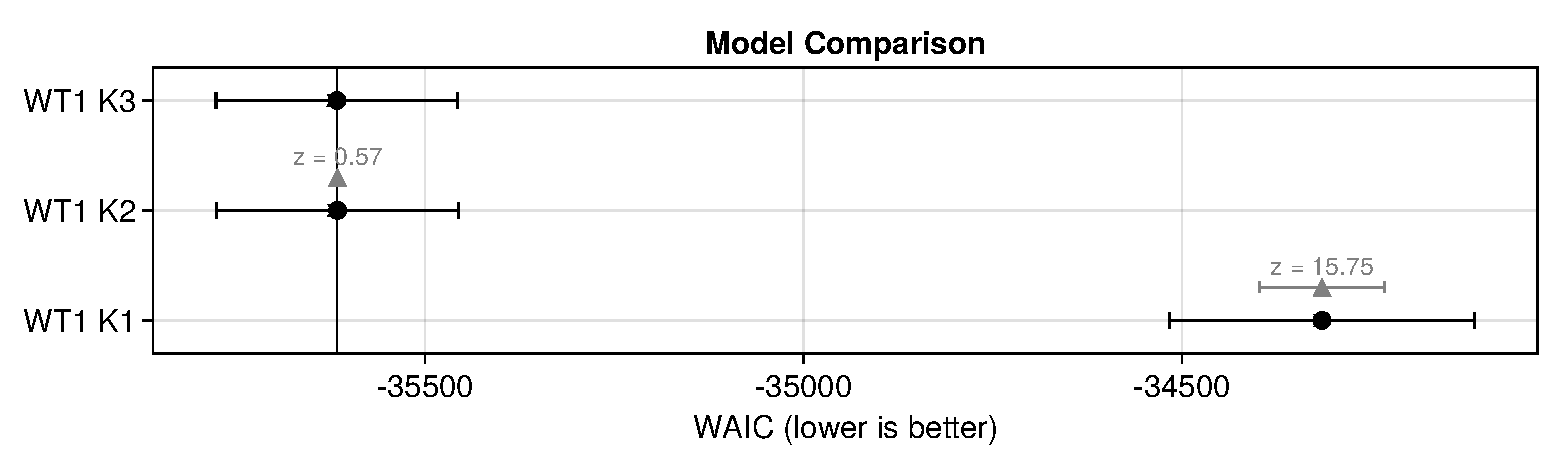
\includegraphics[trim={0mm 0mm 0mm 0mm}, clip, width=\textwidth]{figures/WT1_comparison_waic.pdf}
\end{figure}
